\chapter{Background\label{chap:background}}
\section{The Constant Bandwidth Server theory\label{sec:CBS}}
A Constant Bandwidth Server(CBS) is characterized by a budget $c_s$ and
an pair $(Q_s, T_s)$, where $Q_s$ is the maximum budget and $T_s$
is the period of the server. $U_s = Q_s/T_s$ is called the server bandwidth.
Such a server can be utilized to serve a set of tasks, which can be 
tasks with soft, hard or non real-time guarantee requirements. 
CBS theory defines rules to reserve bandwidth on a single processor.
In our work, we use a hard version of CBS.

For a specific server $S$, at any instant, a fixed deadline $d_{s,k}$ is 
associated with the server. A CBS is said to be active at time $t$ if there 
are pending tasks and $c_s$ is not 0; otherwise it is called idle. 
At any time, among all active servers,
the one with earliest deadline is chosen. Then a served task of this server 
is picked to execute. CBS does not restrict the rule to pick up a particular 
task. For example, first in first out (fifo), rate monotonic scheduling and
any user defined rule can be used.
As the picked task executes, the server budget $c_s$ is decreased by the 
same amount. When budget $c_s$ reaches 0, the server become inactive. At 
each deadline point, the $c_s$ will be recharged to $Q_s$ and a new server 
deadline will be generated as $d_{s, k+1} = d_{s,k} + T_k$. Initially, 
$c_s = Q_s$ and $d_{s, 0} = 0$. When a task arrives at time $t$ and the 
server is idle, if $c_s \ge (d_{s,k} - t)U_s$, the server updates its 
deadline as $d_{s, k+1} = t + T_s$ and $c_s$ is recharged to maximum 
value $Q_s$.

Given a set of servers $\{S_0, S_1, ... , S_n\}$, if
\[
	\sum_{i=0}^n U_i \le 1
\]
then, every $T_i$ time units, a server $S_i$ can obtain $Q_s$ time units 
to serve its tasks. In other words, $U_i$ is the bandwidth a server $S_i$
reserves from a cpu.

\section{The Linux Scheduler\label{sec:LinuxSched}}
A scheduler is responsible for distributing CPU cycles to tasks in the system
according to some scheduling algorithm. In Linux, tasks refer to a process or 
a thread and correspond to the data structure \texttt{struct task\_struct}.
The emphasis in this section is to clarify the relationships and connections
among different scheduling components. As for how each scheduling algorithm 
in Linux is implemented, it's neither the interest of this section or oxc 
framework. To understand the Linux scheduling architecture is the first step 
to explore the oxc framework. For details about how linux schedulers work, 
people can read corresponding chapters in \cite{Wolf} \cite{R.Love}.

\subsection{Scheduling classes\label{sec:LinuxSched_classes}}
Linux scheduling system adapts a modular design, and the basic modularity is
a scheduling class, which is an instance of 
\texttt{struct sched\_class}\footnote{Defined in include/linux/sched.h}. 
Scheduling algorithms are implemented as scheduling classes and a 
scheduling class is a modular scheduler( or simply called a scheduler).
All modular schedulers composes the generic scheduler in Linux.
The \texttt{struct sched\_class} defines a set of interfaces which need to be 
realized in order to implement a scheduler in Linux. These methods are all 
scheduling operations a scheduler in Linux can perform. Each scheduler 
fullfills details behind the interface and carries out its specific
scheduling behaviour. 
There are three scheduling classes in mainline Linux: rt\_sched\_class,
cfs\_sched\_class and idle\_sched\_class\footnote{Defined in rt.c, fair.c, 
and idle.c under kernel/sched directory respectively}. Each scheduling class is 
responsible for scheduling a type of tasks. Tasks scheduled
\texttt{cfs\_sched\_class} are called normal tasks. Tasks scheduled
by \texttt{rt\_sched\_class} are called rt tasks. 
\texttt{idle\_sched\_class} deals with special idles tasks which
does nothing and occupies the CPU when no rt or normal tasks need a CPU.
Now, it's time to see the semantics of scheduling operations for a scheduler.
\begin{lstlisting}[language=C, 
		caption={\texttt{Shceduling operations for a scheduler}},
		label={sched_class}]
struct sched_class {
	const struct sched_class *next;
	void (*enqueue_task) (struct rq *rq, struct task_struct *p, int flags);
	void (*dequeue_task) (struct rq *rq, struct task_struct *p, int flags);
	void (*check_preempt_curr) (struct rq *rq, struct task_struct *p, int flags);
	struct task_struct * (*pick_next_task) (struct rq *rq);
	void (*put_prev_task) (struct rq *rq, struct task_struct *p);
        void (*set_curr_task) (struct rq *rq);
	void (*task_tick) (struct rq *rq, struct task_struct *p, int queued);
	...
};
\end{lstlisting}
\begin{itemize} 
\item \texttt{next:}
	Scheduling classes are linked in a chain, as shown 
	in \ref{fig:sched_classes}.  Whenever a task is needed,
	the scheduler from the beginning to the end of the chain 
	is checked and corresponding scheduling methods are called
	until a task is found. So, schedulers in front have higher 
	priority to execute their tasks. 
\item \texttt{enqueue\_task:}
	Called when a task enters a runnable state. The task is then 
	enqueued into a runqueue, which is an instance of \texttt{struct rq}.
\item \texttt{dequeue\_task:}
	When a task is no longer runnable, this function is called to move
	corresponding task from a runqueue.
\item \texttt{check\_preempt\_curr:}
	This function checks if a task that entered the runnable state 
	should preempt the currently running task.
\item \texttt{pick\_next\_task:}
	This function chooses the task to run next. The newly picked up
	one can be the one currently occupting the CPU; in this case,
	no context switches are needed.
\item \texttt{put\_prev\_task:}
	This is the last scheduling activity for a task before it gives
	up the executing opportunity on a CPU. In fact, it can happen
	that after this operation, the same task still occupies the 
	CPU, as it is picked up again through \texttt{pick\_next\_task}.
\item \texttt{set\_curr\_task:}
	This is the first scheduling operation for a task after a task 
	is chosen to occupy the CPU.
\item \texttt{task\_tick:}
	This function is the most frequently called scheduling function. 
	It is a good point to update the scheduling information, and 
	it might lead to task switch.
\end{itemize} 
\begin{figure}[htbp]
        \centering
        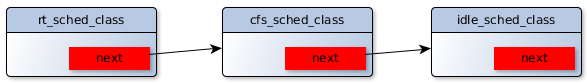
\includegraphics[width=\textwidth]{images/sched_classes}
        \caption{Scheduling classes in Linux}
        \label{fig:sched_classes}
\end{figure}
The basic scheduling unit in Linux is scheduling entity, which can represent
both tasks and task groups. There are two kinds of scheduling entities
\footnote{Both are defined in include/linux/sched.h}:
cfs (scheduling) entities and rt (scheduling) entities.
They are separately defined by \texttt{struct sched\_entity} 
and \texttt{struct sched\_rt\_entity}.
When we say a task is enqueued in a runqueue, more precisely, it is the task's
(cfs or rt) scheduling entity is enqueued.
\begin{lstlisting}[language=C, 
			caption={\texttt{A task embeds scheduling entities}},
			label={task_struct}]
struct task_struct {
	...
	struct sched_entity se;
	struct sched_rt_entity rt;
	...
};
\end{lstlisting}
Both cfs and rt entities are embedded in \texttt{struct task\_struct}. 
For any task, its status can switch between a cfs task and a rt task
through the system call \texttt{sched\_setscheduler}.

When \texttt{CONFIG\_FAIR\_GROUP\_SCHED} is set, cfs task grouping 
is enabled. And \texttt{CONFIG\_RT\_GROUP\_SCHEED} is the kernel configuration
for rt task group scheduling. A task group can contains both rt tasks and
normal tasks, as shown in listing \ref{task_group}. For each CPU, a task group
uses a rt entity and a cfs entity to represent its rt tasks and normal tasks.
Each type of tasks inside a task group is scheduled independently by 
its own scheduling class.
\begin{lstlisting}[language=C,
			caption={\texttt{A task group}},
			label={task_group}]		

struct task_group {
#ifdef CONFIG_FAIR_GROUP_SCHED
	/* sched_entity of this group on each cpu */
	struct sched_entity **se;
	...
#endif
#ifdef CONFIG_RT_GROUP_SCHED
	/* sched_rt_entity of this group on each cpu */
	struct sched_entity **rt_se;
	...
#endif
	...
};
\end{lstlisting}

\subsection{Runqueue centered scheduling\label{LinuxSched_rq}}
Every hook in \texttt{struct sched\_class} deals with the data structure 
\texttt{struct rq}\footnote{Defined in kernel/sched/core.c}, which is called 
runqueue in Linux.  We say that 
Linux scheduling is runqueue centered. In Linux, the \texttt{struct rq} is 
a per CPU data structure; each cpu is associated with a runqueue. Although 
the name indicates, \texttt{struct rq} is not a queue. The \texttt{struct rq}
contains a large amount of information. Its partial contents that are
necessary for understanding this article is listed.
\begin{lstlisting}[language=C,
			caption={\texttt{The runqueue structure}},
			label={runqueue}]
struct rq {
	...
	unsigned long nr_running;
	struct cfs_rq cfs;
	struct rt_rq rt;
	struct task_struct *curr, *idle;
	u64 clock;
	u64 clock_task;
#ifdef CONFIG_SMP
	int cpu;
#endif
	...
};
\end{lstlisting}
\begin{itemize}
\item \texttt{nr\_running} specifies the number of runnable tasks 
	having been enqueued in the runqueue.
\item \texttt{cfs and rt} are two specific runqueues for 
	\texttt{cfs\_sched\_class} and \texttt{rt\_sched\_class} respectively. 
	In order to handle specific type of tasks, different schedulers define 
	new type of runqueue data structures. 
	When we say a task is enqueued into a runqueue, it is finally into
	its corresponding specific runqueue.Each task group has one cfs 
	runqueue and rt runqueue per CPU to enqueue the tasks and sub task
	groups it contains in that CPU. 
	Figure \ref{task_group1} adds this new information to the
	knowledge just introduced for a task group, as in 
	figure \ref{task_group}. The default task group in the system points
	their cfs runqueue and rt runqueue to fields contained in the
	per CPU runqueue directly. 
\item \texttt{curr} points to the task currently running in this runqueue.
\item \texttt{idle} points to a special idle task. This is the task occupying
		the CPU  when no other tasks are runnable.
\item \texttt{clock and clock\_task} are time information kept by the runqueue.
	They updated by \texttt{update\_rq\_clock} method and some scheduling
	operation can rely them as time source.
\item \texttt{cpu} tells the CPU of this runqueue.
\end{itemize}
\begin{lstlisting}[language=C,
caption={\texttt{Specific runqueue information within a task group}},
			label={task_group1}]		

struct task_group {
#ifdef CONFIG_FAIR_GROUP_SCHED
	/* sched_entity of this group on each cpu */
	struct sched_entity **se;
	/* runqueue "owned" by this group on each cpu */
	struct cfs_rq **cfs_rq;
	...
#endif
#ifdef CONFIG_RT_GROUP_SCHED
	/* sched_rt_entity of this group on each cpu */
	struct sched_entity **rt_se;
	struct rt_rq **rt_rq;
	...
#endif
	...
};
\end{lstlisting}

\subsection{Completely Fair scheduler\label{sec:LinuxSched_cfs}}
Completely fair scheduler is implemented in \texttt{fair\_sched\_class}. 
Most tasks inside Linux are scheduled by completely fair scheduling class
and are normal tasks, which can be further divided into three sub 
types given scheduling policies (\texttt{SCHED\_NORMAL}, \texttt{SCHED\_BATCH}
and \texttt{SCHED\_IDLE\footnote{This SCHED\_IDLE policy is not related to
idle\_sched\_class which aims to handle a special idle task.}}).

CFS tries to distribute CPU cycles fairly to tasks and task groups according
to their \emph{weight}. A specific runqueue structure \texttt{struct cfs\_rq}
is provided to deal with normal tasks. 
Recall that an instance of such cfs runqueue is embedded in the per 
CPU runqueue and each task group holds a pointer
to cfs runqueue on each CPU to store cfs tasks belonging to it.
A little more details on cfs runqueue and cfs scheduling entity are followed.
%The scheduling entity handled by cfs scheduling class is 
%\texttt{struct sched\_entity}. Here instead of studying the details of
%CFS, we are going to see how different scheduling components
\begin{lstlisting}[language=C,
		caption={\texttt{The cfs runqueue}},
		label={cfsrunqueue}]
struct cfs_rq {
        unsigned long nr_running;
        struct rb_root tasks_timeline;
#ifdef CONFIG_FAIR_GROUP_SCHED
        struct rq *rq;  
	struct task_group *tg;
#endif
	...
};
\end{lstlisting}
\begin{itemize}
\item \texttt{nr\_running} is the number of cfs tasks(entities) in this cfs 
	runqueue.
\item \texttt{tasks\_timeline} is the root of the red-black tree 
	\cite{rbtree} where 
	all cfs entities enququed into this cfs runqueue is stored. 
	This article will not go into details of the red-black tree
	mechanism, people only need to know it is an efficient way 
	to sort and access data elements.
\item \texttt{rq} is the per CPU runqueue that the task group \texttt{tg} 
	is finally enqueued.
\item \texttt{tg} is the task group that owns this cfs runqueue.
\end{itemize}
\begin{lstlisting}[language=C,
			caption={\texttt{The cfs scheduling entity}},
			label={sched_entity}]
struct sched_entity {
	...
	struct cfs_rq *cfs_rq;
#ifdef CONFIG_FAIR_GROUP_SCHED
	struct cfs_rq *my_q;
#endif
	...
}; 
\end{lstlisting}
\begin{itemize}
\item \texttt{cfs\_rq} is where this entity is to be queued.
		
\item \texttt{my\_rq} is the cfs runqueue owned by this entity(group).
	Remember that a scheduling entity can also represent a task group.
\end{itemize}
Now there is enough information to show how different scheduling components
(\texttt{sched\_entity}, \texttt{task\_struct}, \texttt{task\_group}
and \texttt{struct cfs\_rq}) are related in completely fair scheduler.

In this case that cfs task group scheduling is enabled. the cfs scheduling 
scheme is shown in figure\ref{fig:cfs_scheme_tg}. 
This is not a complete scheme: 1) Under a task group there could be sub groups, which behave as the task in the figure 2) In the system, there is a top group, 
which includes all tasks in the system by default; tasks in this group are 
enqueued in the cfs runqueue embedded in the per CPU runqueue directly.
\begin{figure}[htbp]
        \centering
        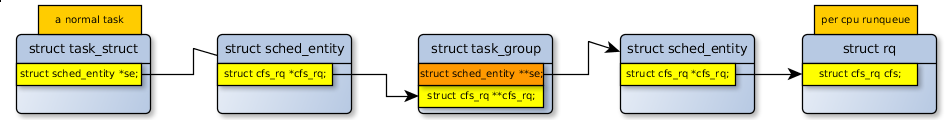
\includegraphics[width=\textwidth]{images/cfs_scheduling_scheme_tg}
        \caption{CFS scheduling when cfs group scheduling is enabled.}
        \label{fig:cfs_scheme_tg}
\end{figure}

If cfs task group scheduling is not enabled, a task is directed to its 
per CPU runqueue by a \emph{task\_rq} marco. \emph{task\_rq} also works 
for rt tasks when rt task group scheduling is not enabled.
\ref{fig:cfs_scheme_no_tg}.
\begin{figure}[htbp]
        \centering
        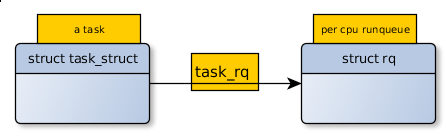
\includegraphics[height=0.1\textheight,width=0.5\textwidth]{images/scheduling_scheme_no_tg}
        \caption{Scheduling scheme without group scheduling}
        \label{fig:cfs_scheme_no_tg}
\end{figure}

We call the scheme in figure \ref{fig:cfs_scheme_tg} and 
\ref{fig:cfs_scheme_no_tg} \emph{scheduling routes} in cfs scheduling. 
The route source is a task and the destination is a runqueue. 
The feature of a scheduling route is that if one component in the route 
is known, then other scheduling components in the direction towards the 
destination can be tracked.
The concept of scheduling route is first invented in our work. 
Later you will see the theory behind oxc framework explores scheduling routes
in Linux extensivly. We believe a new concept is deserved in formalizing 
the work for oxc framework.

\subsection{Real time scheduler\label{sec:LinuxSched_rt}}
Tasks with POSIX real time policies \texttt{SCHED\_FIFO} and \texttt{SCHED\_RR}
are scheduled by the real time scheduling class \texttt{rt\_sched\_class} and
are called rt tasks. Given figure\ref{fig:sched_classes}, rt tasks are always
schedueld over normal tasks. 

\texttt{SCHED\_FIFO} implements a simple first-in, first-out scheduling 
algorithm. A running \texttt{SCHED\_FIFO} task can only be preempted by a 
higher priority rt task. \texttt{SCHED\_RR} is \texttt{SCHED\_FIFO} with 
timeslices --- it is a round robin algrithm. When a \texttt{SCHED\_RR}
task exhausts its timeslice, another \texttt{SCHED\_RR} task of the same
priprity is picked to run a timeslice, and so on. In either case, a rt task
cannot be preempted by a lower priority task.

The rt scheduling class provides with a sub runqueue structure 
\texttt{struct rt\_rq} to deal with rt tasks.
\begin{lstlisting}[language=C,
		caption={\texttt{The rt runqueue}},
		label={rtrunqueue}]
struct rt_rq {
	struct rt_prio_array active;
        unsigned long rt_nr_running;
#ifdef CONFIG_RT_GROUP_SCHED
        struct rq *rq;
        struct task_group *tg;
#endif
	...
};

struct rt_prio_array {
	DECLARE_BITMAP(bitmap, MAX_RT_PRIO+1); 
	struct list_head queue[MAX_RT_PRIO];
};
\end{lstlisting}
All rt tasks with the same priority, let's say $prio$, are kept in a linked 
list headed by $active.queue[prio]$. If there is a task in the list, the 
corresponding bit in $active.bitmap$ is set. All other fields have the same
meaning as in cfs runqueue. Compare with the cfs scheduling entity, the 
following \texttt{struct sched\_rt\_entity} is self explanatory enough. 
\begin{lstlisting}[language=C,
		caption={\texttt{The rt scheduling entity}},
		label={rt_entity}]
struct sched_rt_entity {
	...
	struct rt_rq *rt_rq;
#ifdef CONFIG_RT_GROUP_SCHED
	struct rt_rq *my_q;
#endif
	...
}; 
\end{lstlisting}

%The connections among \texttt{struct sched\_rt\_entity} and other scheduling
%components are similar to the \text{struct sched\_entity} case.
When \texttt{CONFIG\_RT\_GROUP\_SCHED} is set, figure\ref{fig:rt_scheme_tg} 
shows the scheduling route for rt scheduling. If rt task group scheduling is 
not enabled, still \emph{task\_rq} marco will be used.
\begin{figure}[htbp]
        \centering
        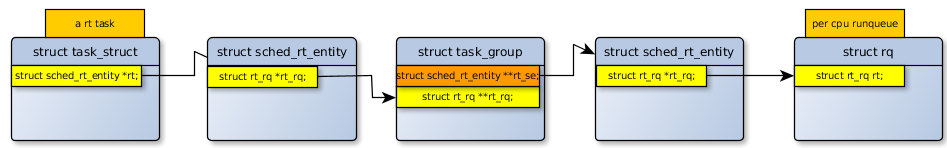
\includegraphics[width=\textwidth]{images/rt_scheduling_scheme_tg}
        \caption{RT scheduling when rt group scheduling is enabled.}
        \label{fig:rt_scheme_tg}
\end{figure}

\section{Related work\label{sec:RelatedWork}}
\subsection{RT throttling\label{sec:RelatedWork_RT}}
Enabling \texttt{CONFIG\_RT\_GROUP\_SCHED} lets users explicitly allocate
CPU bandiwidth to rt tasks in task groups. It uses the \emph{control group}
(cgroup) virtual file system. Each cgroup associates a set of tasks with
a set of resources, called \emph{subsystems}. For example \emph{cpuset} 
subsystem is responsible for assigning a set of CPUs and Memory Nodes to
tasks in a cgroup. Such tasks and resources can be further distributed in 
sub cgroups. Each cgroup is represented by a directory in the cgroup file 
system and a hierarchy of cgroups maps to a hierarchy of directories. In 
the directory, each mounted subsystem provides a list of files that are used 
as interfaces to control the allocation of a resource.
Through mounting the \emph{cpu} subsystem, two interfaces $cpu.rt\_period\_us$ 
and $cpu.rt\_runtime\_us$ are used to control the CPU bandwidth for rt 
tasks in each cgroup. That is, the total execution time of rt tasks in a cgroup 
on each CPU in time length $rt\_period\_us$ cannot exceed $rt\_runtime\_us$. 
If this constraint is met, rt tasks would not be choosen to run on that CPU 
until a new period; we call such tasks be throttled.

No matter \texttt{CONFIG\_RT\_GROUP\_SCHED} is set or not, in order to avoid rt 
tasks forever occupy thc CPU, there is a system wide setting that constraints
rt tasks' execution through the /proc virtual file system :

	$/proc/sys/kernel/sched\_rt\_period\_us$ 

	$/proc/sys/kernel/sched\_rt\_runtime\_us$ 
\\This applies to all rt tasks in a system.

\subsection{CFS bandwidth control\label{RelatedWork_CFS}}
Basically, CFS bandwidth control is the same technique as RT throttling
applying on normal tasks. It is a \texttt{CONFIG\_FAIR\_GROUP\_SCHED} 
extension which allows the specification of the maximum CPU bandwidth
available to normal tasks  in a cgroup or cgroup hierarchy.
The bandwidth allowed to a cgroup is specified using a 
quota(\texttt{cpu.cfs\_quota\_us}) and a period(\texttt{cpu.cfs\_period\_us}).
By specifying this, normal tasks in a cgroup will be limited to 
\texttt{cfs\_quota\_us} units of CPU time within the period of 
\texttt{cfs\_period\_us}. Recall that in RT throttling \ref{sec:RelatedWork_RT},
the reserved bandwidth through cgroup interfaces are applied in each CPU
individually.
\subsection{AQuoSA\label{sec:AQuoSA}}
The Adaptive Quality of Service Architecture composes two parts: 
a resource reservation scheduler an a feedback-based
control mechanism. The scheduler uses CBS rules to rserve CPU bandwidth for
a task, which is a rt task with SCHED\_RR policy in its Linux implementation.
Given the error between the reserved computation and the amount of CPU cycles
really consumed, the feedback controller adapts CBS reservation paramters to
provide quality of service CPU allocation in the system.
The control mechanism depends on CBS performance, not the scheduling details.
That is, such a control mechanism can be applied to general CBS based 
scheduling. AQuoSA lacks considerations on multi-processor platform.
  
\subsection{Schedule-deadline patch}
The schedule-deadline patch for Linux kernel is being developed to extend
current mainline Linux with a deadline-based scheduling method. 
In schedule-deadline, a new scheduling class (scheduler) is implemented and 
has highest priority among all scheduling classes. Tasks scheduled by this
scheduling class are called sched tasks. A sched task is assigned deadlines
according to CBS rules and scheduled in ''earliest deadline first (EDF)'' way.
\subsection{IRMOS real-time framework}
The rague name IRMOS comes from the European project ''Interactive Real-time
Multimedia Applications on Service Oriented Infrastructures''. 
The IRMOS 
framework replace rt throttling mechanism in mainline Linux with real time
CPU reservation(still CBS), and reuses the existing interfaces. So, users 
configure the cgroup interface as what we saw in rt 
throttling(\ref{sec:RelatedWork_RT}), the difference is that this time the CPU 
bandwidth is allocated in a guaranteed way. Also, new cgroup interfaces are 
added to assist reserved CPU power distribution in the cgroup hierarchy.
